\chapter{基于预训练辅助模型的Token表征学习}
\label{chap:Token}
本章主要对本文提出的基于预训练辅助模型的Token表征学习方法进行详细介绍,首先介绍其研究动机,接着阐述其方法设计,以及具体的实现过程,最后介绍实验验证过程和结果。

\section{研究动机}
\label{sec:TokenMotivation}

基于Token的代码表征方法本质上就是将源代码转换为一系列词法单元Token组成的序列,并对Token序列进行代码分析。基于Token的代码表征方法存在两种主要限制:

(1)集外词问题:类似于自然语言技术处理文本,由于源代码中存在大量用户自己定义的标识符,不同用户的命名习惯不同,在对源代码的词法单元建模时,会产生一个规模巨大且稀疏的词汇表。该词汇表的规模会直接影响代码分析任务的效率,因此现有方法大多都对Token进行规范化,比如将变量名用统一的标识符来代替,从而降低词汇表的规模。但是后续神经网络模型训练过程中,当出现某个词汇在词汇表中没有出现过,那么神经网络模型就无法对齐建模,即出现了在词汇表中不存在的Token,集外词(Out-of-vocabulary,简称OOV)问题。有研究\cite{RJXB202205011}发现,针对代码表征中的集外词问题,在经典BigcloneBench\cite{7332459}数据集中OOV比率高达62.68\%,在OJClone数据集\cite{WOS:000485474201046}中OOV比率达到了16.82\%。

(2)预训练辅助模型训练代价大:为了解决OOV问题,本文打算使用预训练模型增加词汇表的大小。近期,研究人员在大规模语料库上预训练各种语言模型,在解决各种自然语言处理任务方面取得了良好进展\cite{zhao2023survey}。在表征学习领域,也有基于大规模预训练模型提升代码表征能力的方法被提出。InferCode\cite{9402028}将自然语言处理中的自监督学习思想引入到代码的抽象语法树的表示中, 通过预测从AST上下文中自动识别的子树来训练代码表征,并且使用AST的子树作为训练标签,从而无需任何人工标记工作。该预训练InferCode模型可以应用于下游的无监督学习,例如代码聚类、代码克隆检测、跨语言代码搜索等。GraphCodeBERT\cite{guo2021graphcodebert}方法提出了一个基于数据流的代码表征预训练模型,与抽象语法树不同,数据流包含代码变量间“值从哪里来”的语义特征,并不会带来深层次不必要的复杂信息,使用该特征可以更有效的生成代码表征。然而这些预训练模型通常存在参数规模庞大, 训练及使用代价大的问题。

因此,针对集外词OOV问题,本文提出了一种轻量级的基于预训练辅助模型的Token表征学习方法,该方法在提升代码表征能力的同时,并不会引入过多参数,造成模型训练代价高的问题。

\section{Token表征方法设计}
\label{sec:Token}
本节将主要介绍基于预训练辅助模型的Token表征学习方法的详细设计,首先介绍该方法的整体框架,并分别从预训练辅助词嵌入、Token代码表征两方面介绍具体设计。

\subsection{框架概述}
\label{subsec:TokenOverview}
本文提出的基于预训练辅助模型的Token表征学习方法整体框架如图\ref{fig:tokenframework}所示。该框架的输入是代码片段对应的Token序列,输出是对应的属性特征向量,主要包括预训练辅助词嵌入、Token代码表征两个阶段。

\begin{figure}[H]
  \centering
  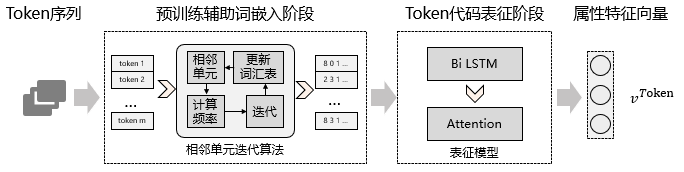
\includegraphics[width=0.95\textwidth]{figures/tokenframework}
  \caption{基于预训练辅助模型的Token表征学习框架}\label{fig:tokenframework}
\end{figure}

首先,预训练辅助词嵌入阶段以代码片段的Token序列作为训练数据,构建一个预训练辅助词嵌入模型。该模型的输入是代码片段对应的Token序列,输出为与输入对应的Token词嵌入向量。然后通过对模型的训练,使得该模型具有正确识别Token的能力,并将该模型保存下来。需要注意的是,为了减少集外词OOV问题,本文对模型采用相邻单元迭代算法,即,通过多次迭代来更新词汇表。

其次,Token代码表征阶段以Token词嵌入向量作为训练数据,构建一个Token表征模型。该模型的输入是Token序列对应的词向量,输出为一个固定长度的密集向量用来表示代码的属性特征。需要注意的是,本文选用的AttBiLSTM神经网络,主要包含两个部分:双向长短时记忆部分(BiLSTM)和自注意力机制部分(Attention),前者主要目的是同时捕获序列的双向语义信息,后者的主要目的是总结序列的输入特征,并将每个代码片段缩减为一个单一的密集向量。

在上述框架中,本文的创新点主要体现在预训练辅助词嵌入阶段的相邻单元迭代算法、Token代码表征阶段的模型设计两方面,下面将围绕这两个创新点来阐述本文的方法。

\subsection{预训练辅助词嵌入设计}
\label{subsec:TokenPreModel}

与自然语言处理类似,源代码的词法单元Token可以视为句子中的单词,Token维度的代码表征方法第一步就是将词法单元Token转换为机器易于理解和操作的数值向量,即词嵌入技术。它将词汇表中的每个单词转换成一个低维度、连续的向量表示,这种向量通常被称为词向量。目前,使用预训练词嵌入模型训练词向量的研究工作发展迅速,Word2vec、GloVe、FastText、ELMo和BERT等模型也相继被提出。其中,Word2vec模型通过从大规模无标注文本数据集中学习上下文信息,自动捕捉并编码词汇的语义关系,生成的词嵌入向量作为下游任务的输入特征,可以显著提升神经网络模型的性能和泛化能力。因此,本文采用Word2vec模型进行词嵌入。

同时,为了减少集外词OOV问题出现的概率,本文提出了一种相邻单元迭代算法(Adjacent token iterative algorithm,简称ATIA),该算法通过组合Token序列中相邻单元构造新的代码表示单元,然后统计新单元出现的频率,根据频率信息多次迭代,不断更新词汇表。下面对相邻单元迭代算法进行介绍。

具体地,首先将代码数据集中的源代码经过代码预处理,得到对应的Token序列作为初始语料库,代码预处理的工作详见\ref{subsec:Preprocess}节,这里不展开阐述。然后按照代码块组合相邻Token并查找出出现次数最频繁的Token组合,将这个组合称为新的迭代单元(Adjacent gram,简称Agram)。最后将这个Agram当作新的独立单元,加入到词汇表中,而原本组成这个Agram的原始Token单元并不会从词汇表中删除。在第一次迭代的时候,选取相邻的两两Token作为组合,把出现最频繁的Token组合确定为一个Agram单元之后再进行二次迭代,每次迭代在原来的基本单元上再组合一个新的邻近Token作为新的判断单元,不断的进行迭代,每次迭代都要对应的更新词汇表。

相邻单元迭代算法ATIA的伪代码如\ref{alg1}所示。该算法有两个输入:待处理的初始Token语料库$Corpus$、迭代次数$N$,有两个输出:经过多次迭代后生成的语料库$NewCorpus$、词汇表$Vocab$,具体包括初始化AgramsSet、计算单元Agram出现的次数、更新语料库3个步骤,每个步骤的作用如下:

\begin{algorithm}[ht]  
	\renewcommand{\algorithmicrequire}{\textbf{Input:}}
	\renewcommand{\algorithmicensure}{\textbf{Output:}}
	\caption{Iterative algorithm}  
	\label{alg1}
	\begin{algorithmic}[1]
    \Require Origin Tokens Corpus:$Corpus$
    \Require The number of iterations:$N$
		\Ensure New Corpus: $New\_Corpus$
    \Ensure Vocabulary:$Vocab$
    \State $AgramsSet = \varnothing $ 
    \State $New\_Corpus \leftarrow Corpus $ 
    \State $Vocab = \left\{\right\} $  \Comment{step1:初始化}
		\For{$i \leftarrow 1$ to $N$}
      \If {i == 1}
        \For{token $in$ Corpus}
          \State add adjacent token to AgramsSet
        \EndFor 
      \Else
        \State numbers[] = \{\} 
        \For{Agram $in$ Aragms}
          \State Calculate the number of Argram in Corpus 
          \State add number to numbers \Comment{step2:计算单元Agram出现的次数} 
        \EndFor 
        \State $n \leftarrow $ Max(numbers) 
        \State $Max\_Agram \leftarrow$ Agram in Agrams whose number is n
        \State add $\left(Max\_Agram:n\right)$ to Vocab \Comment{step3:更新词汇表}
        \State add Agram to New\_Corpus \Comment{step3:更新语料库}
      \EndIf
    \EndFor \\
    \Return $New\_Corpus,Vocab$ 
	\end{algorithmic}
\end{algorithm}

(1)初始化:首先初始化一个AgramsSet用来存放Token组合,初始化一个词汇表用来存放Token及其出现次数,并且将目前已有的Token语料库$Corpus$添加进$NewCorpus$。

(2)计算单元Agram出现的次数:多次迭代,在第一次迭代时,组合相邻Token,得到Agram组合,并添加进AragmsSet集合中。遍历语料库,计算AgramsSet中所有的Aragm出现的次数,并且把Aragm组合当作key,组合出现的次数当作对应key的value值保存到词汇表。

(3)更新:遍历AragmsSet中所有的Agram的value值,将频率最高的Agram合并到新语料库中。然后重复(2)、(3)步骤,直到迭代次数N减少为0。

\subsection{Token代码表征设计}
\label{subsec:TokenModel}
(1)结构设计

为了提高Token维度代码表征能力,本文选用AttBiLSTM神经网络对上述得到词向量进行建模,具体的模型设计如图\ref{fig:tokenmodel}所示。该模型主要包括输入层、双向长短时记忆层(BiLSTM)和自注意力机制层(Attention)、输出层。
\begin{figure}[H]
  \centering
  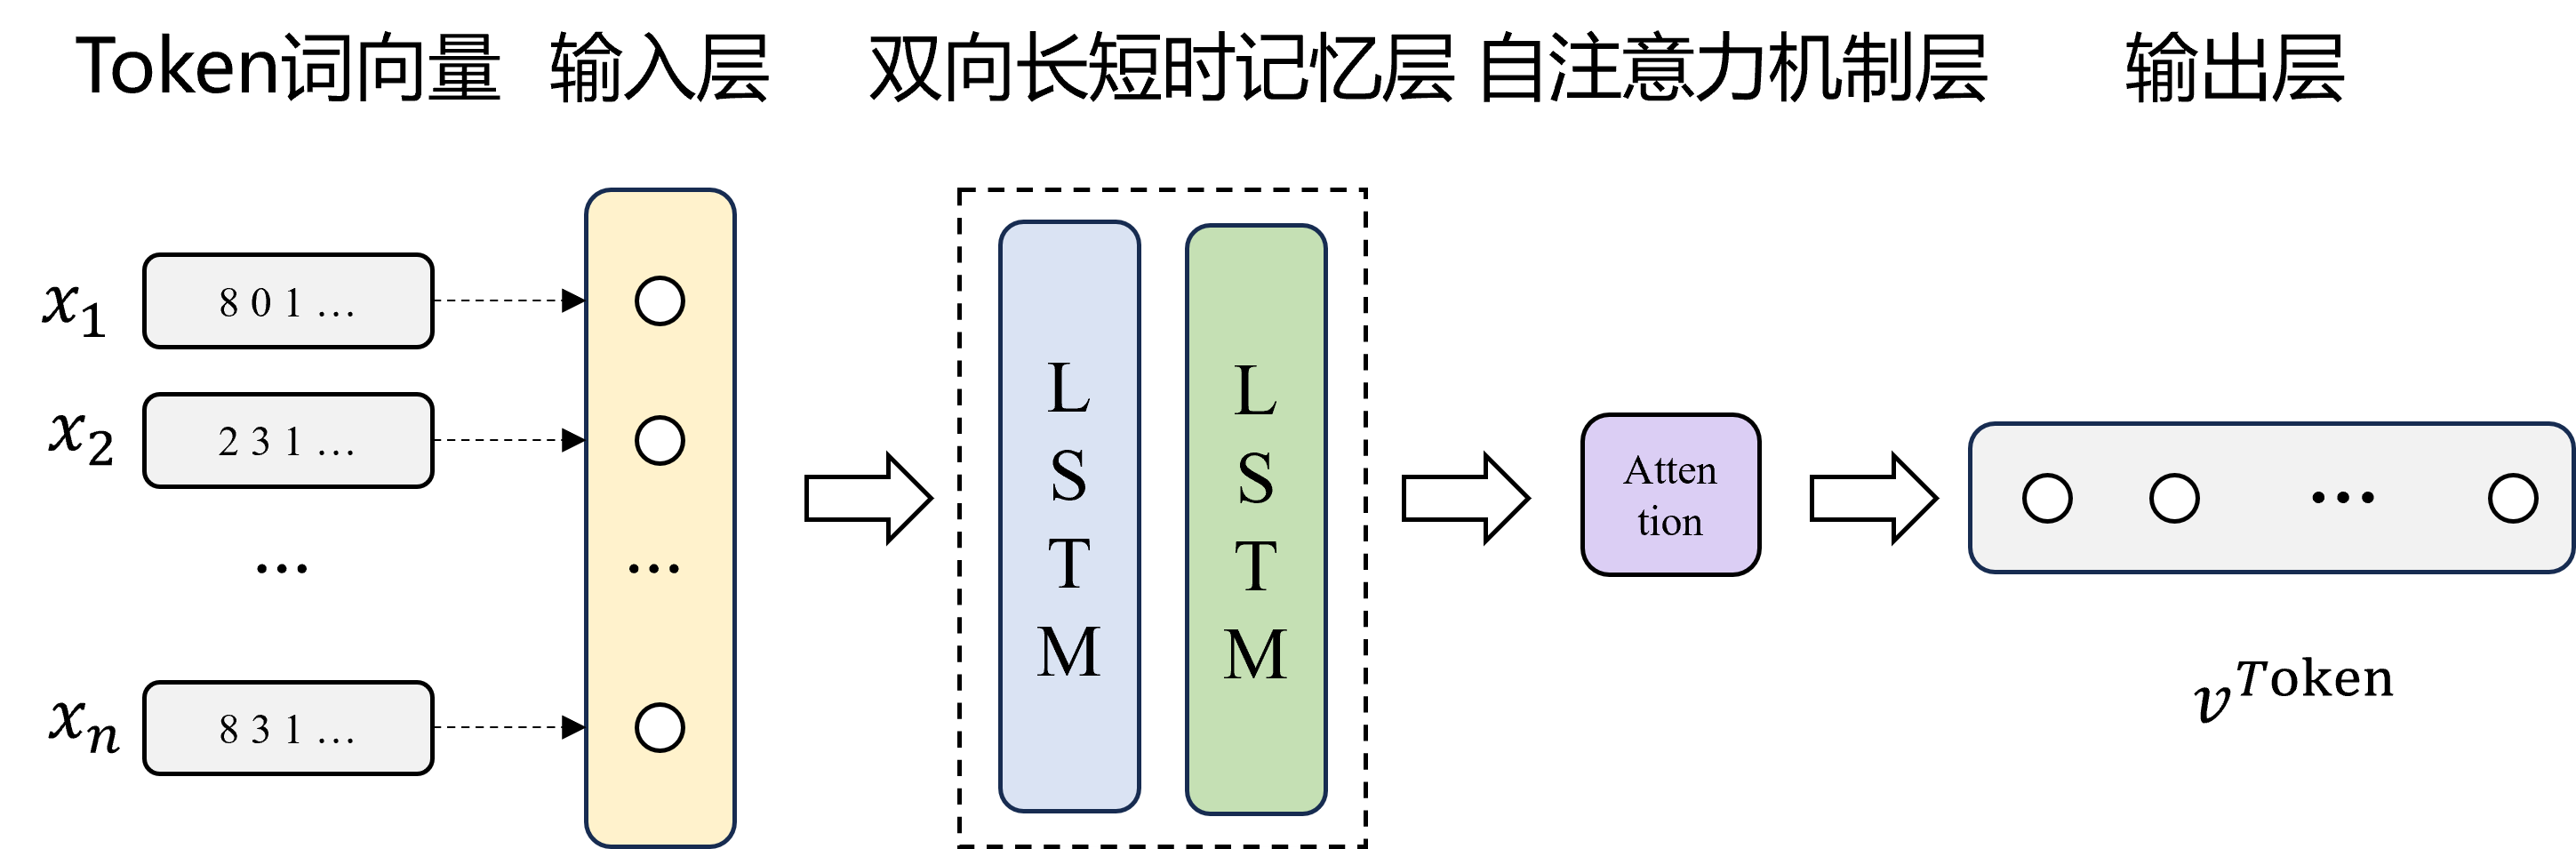
\includegraphics[width=0.85\textwidth]{figures/tokenmodel}
  \caption{Token代码表征:AttBiLSTM模型设计}\label{fig:tokenmodel}
\end{figure}

\ding{172}输入层:输入层用于向模型输入训练数据,在本方法中模型的输入为经过预训练辅助嵌入模型得到的Token序列词向量,即每个词向量对应一个输入神经元。\ding{173}双向长短时记忆层:由两层LSTM构成,同时捕获序列的双向语义信息。\ding{174}自注意力机制层:本层的主要目的是总结序列的输入特征,并将每个代码片段缩减为一个单一的密集向量。\ding{175}输出层:每个Token序列对应一个输出。

(2)模型选型

考虑到代码的Token序列是一种序列化的输入,并且前后词法单元可能存在依赖关系,目前常见的学习序列中长依赖关系的递归神经网络模型为长短期记忆网络LSTM,其时序结构如下图\ref{fig:LSTM}所示。每一个LSTM单元都有一个细胞状态和三个门(输入、输出、遗忘),通过三个门调节信息的流动,控制输入、自身状态、输出所占的比重,使网络能够在长时间内保留或遗忘信息。
\begin{figure}[H]
  \centering
  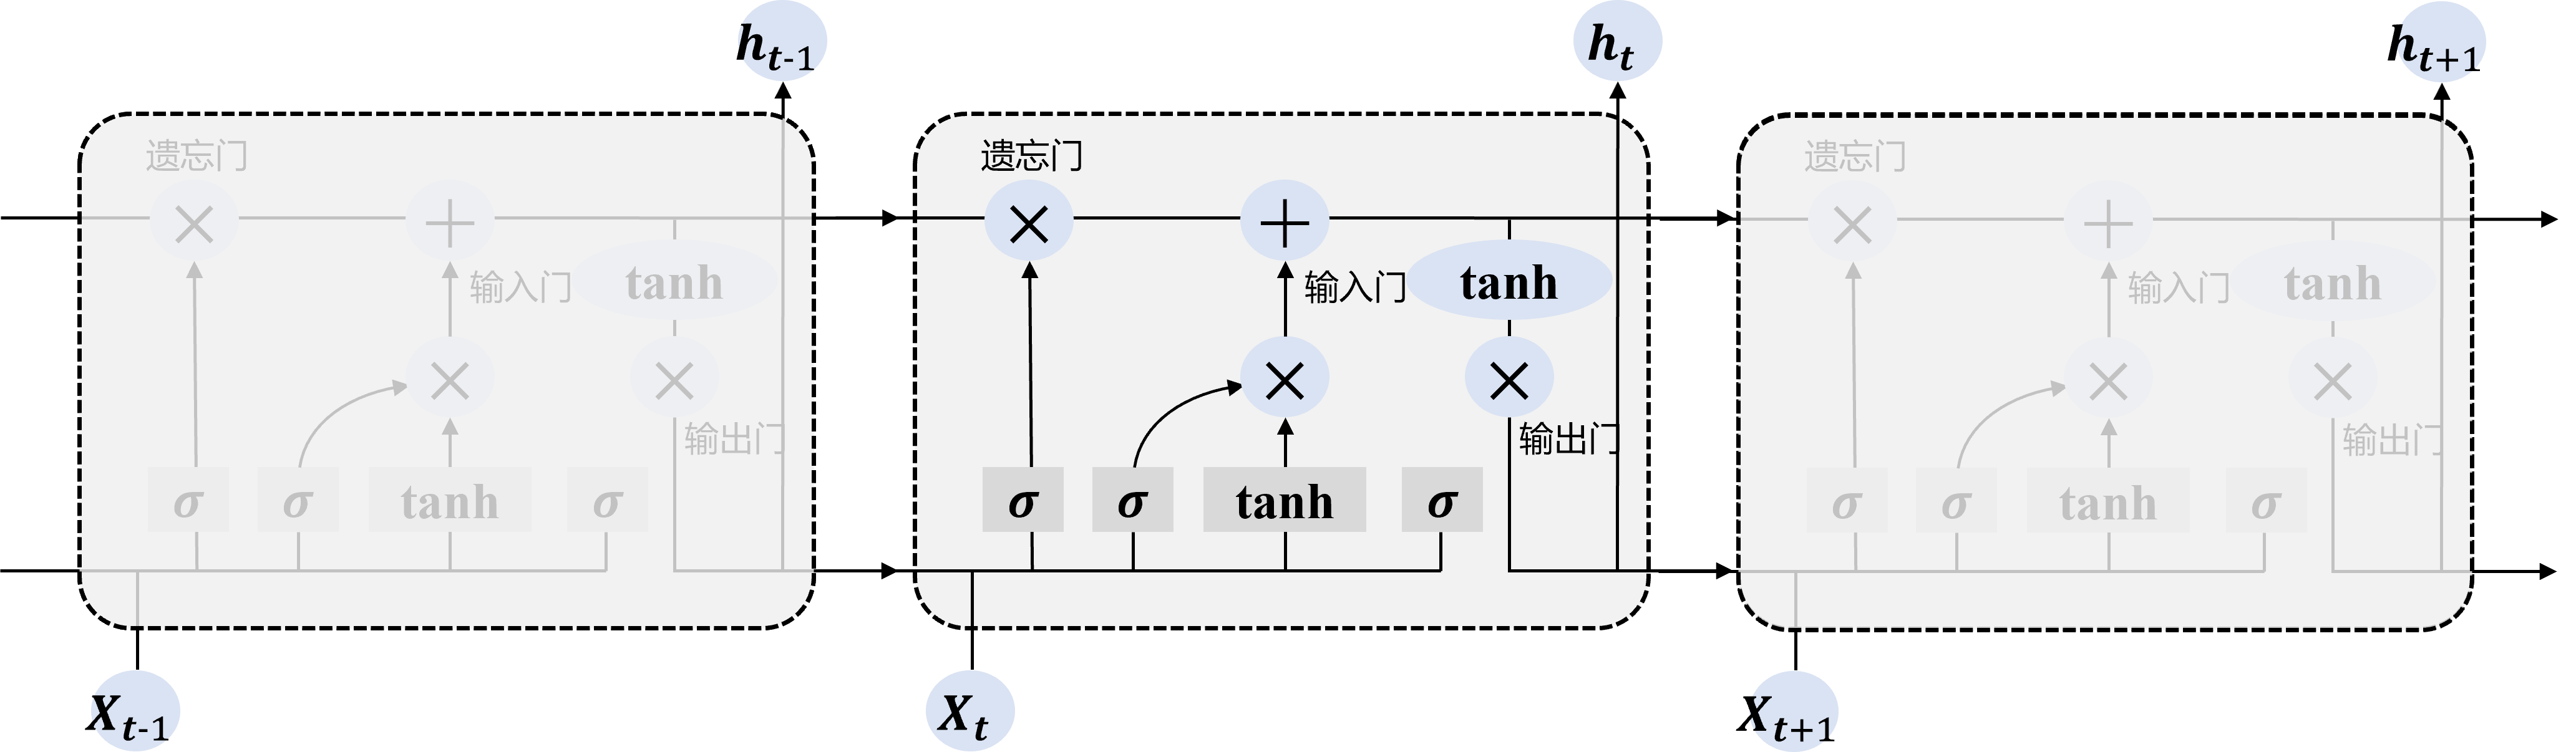
\includegraphics[width=0.85\textwidth]{figures/LSTM}
  \caption{LSTM模型时序结构图}\label{fig:LSTM}
\end{figure}

具体来说,第一步需要接受上一个时间步的隐藏状态$h_{t-1}$和当前时间步的输入数据$x_{t}$,输入遗忘门。遗忘门用来决定在当前时间步的存储状态中传递哪些前一个时间步的信息。具体地,将合并的结果通过矩阵相乘、加偏置、非线性转换,得到一个介于0到1之间的输出值$f_{t}$,通过公式\ref{e3.1}决定是否需要保留和遗忘多少信息,其中$\sigma$表示为非线性激活sigmoid函数,得出的值越接近0越有可能被丢弃,越接近1越有可能被记住。
\begin{equation}\label{e3.1}
  \begin{split}
    f_{t} = \sigma \left(W_{f} \cdot \left[h_{t-1},x_{t}\right] + b_f \right)
  \end{split}
\end{equation}

输入门用来确定输入的$x_{t}$中哪些信息能够传递到当前时间步,具体的计算公式如\ref{e3.2},同时依赖于$tanh$ 和 $sigmoid$函数,得到当前时间步中需要记录的值$\widetilde{C_t}$。
\begin{equation}\label{e3.2}
  \begin{split}
    i_t &= \sigma \left(W_{i} \cdot \left[h_{t-1},x_{t}\right] + b_i\right)
    \\
    \widetilde{C_t} &= \tanh \left(W_{c} \cdot \left[h_{t-1},x_{t}\right] + b_c \right)
  \end{split}
\end{equation}

为了更新新旧细胞的状态,使用公式\ref{e3.3}计算当前时刻细胞的最终状态$C_t$。具体地,用$f_{t}$来控制丢弃旧细胞信息,同时加上新的重要信息。
\begin{equation}\label{e3.3}
  \begin{split}
   C_t = f_t \otimes C_{t-1} + i_t \otimes \widetilde{C_t}
  \end{split}
\end{equation}

输出门用来确定当前时间步的信息有多少能够传递到下一个时间步,具体的计算公式如\ref{e3.4}。
\begin{equation}\label{e3.4}
  \begin{split}
   out_t &= \sigma \left(W_{out} \cdot \left[h_{t-1},x_{t}\right] + b_o \right)
   \\
   h_t &= out_t \otimes \tanh \left(C_t\right)
  \end{split}
\end{equation}

通过上述三个门的时序操作,最终得到长期状态$C_t$和短期记忆$h_t$。长期状态$C_t$从左到右经过LSTM单元,通过遗忘门丢失一些前时间步信息,通过输入门添加当前时间步信息,最后通过输出门输出。但LSTM模型存在一个问题,即无法获取从后往前的信息。

为了更好地提高模型对Token序列数据的表征能力,本文选择了双向长短期记忆网络BiLSTM模型来进行Token代码表征,模型的结构如图\ref{fig:BiLSTM}所示。BiLSTM模型由一个正向的LSTM模型和一个反向的LSTM模型组成,主要思想是通过把序列向前、向后分别输入给两个独立的递归网络,这两个子网络连接到一个输出层,在每个词的输出部分把两个子网络的输出信息进行整合,这样网络就同时拥有了序列中每个词的过去时刻信息和未来时刻信息,更全面地捕捉序列信息,从而提高模型的性能。BiLSTM可以捕获到序列前后的关系依赖,将代码片段的Token序列转换为可相互比较的向量。
\begin{figure}[H] 
  \centering
  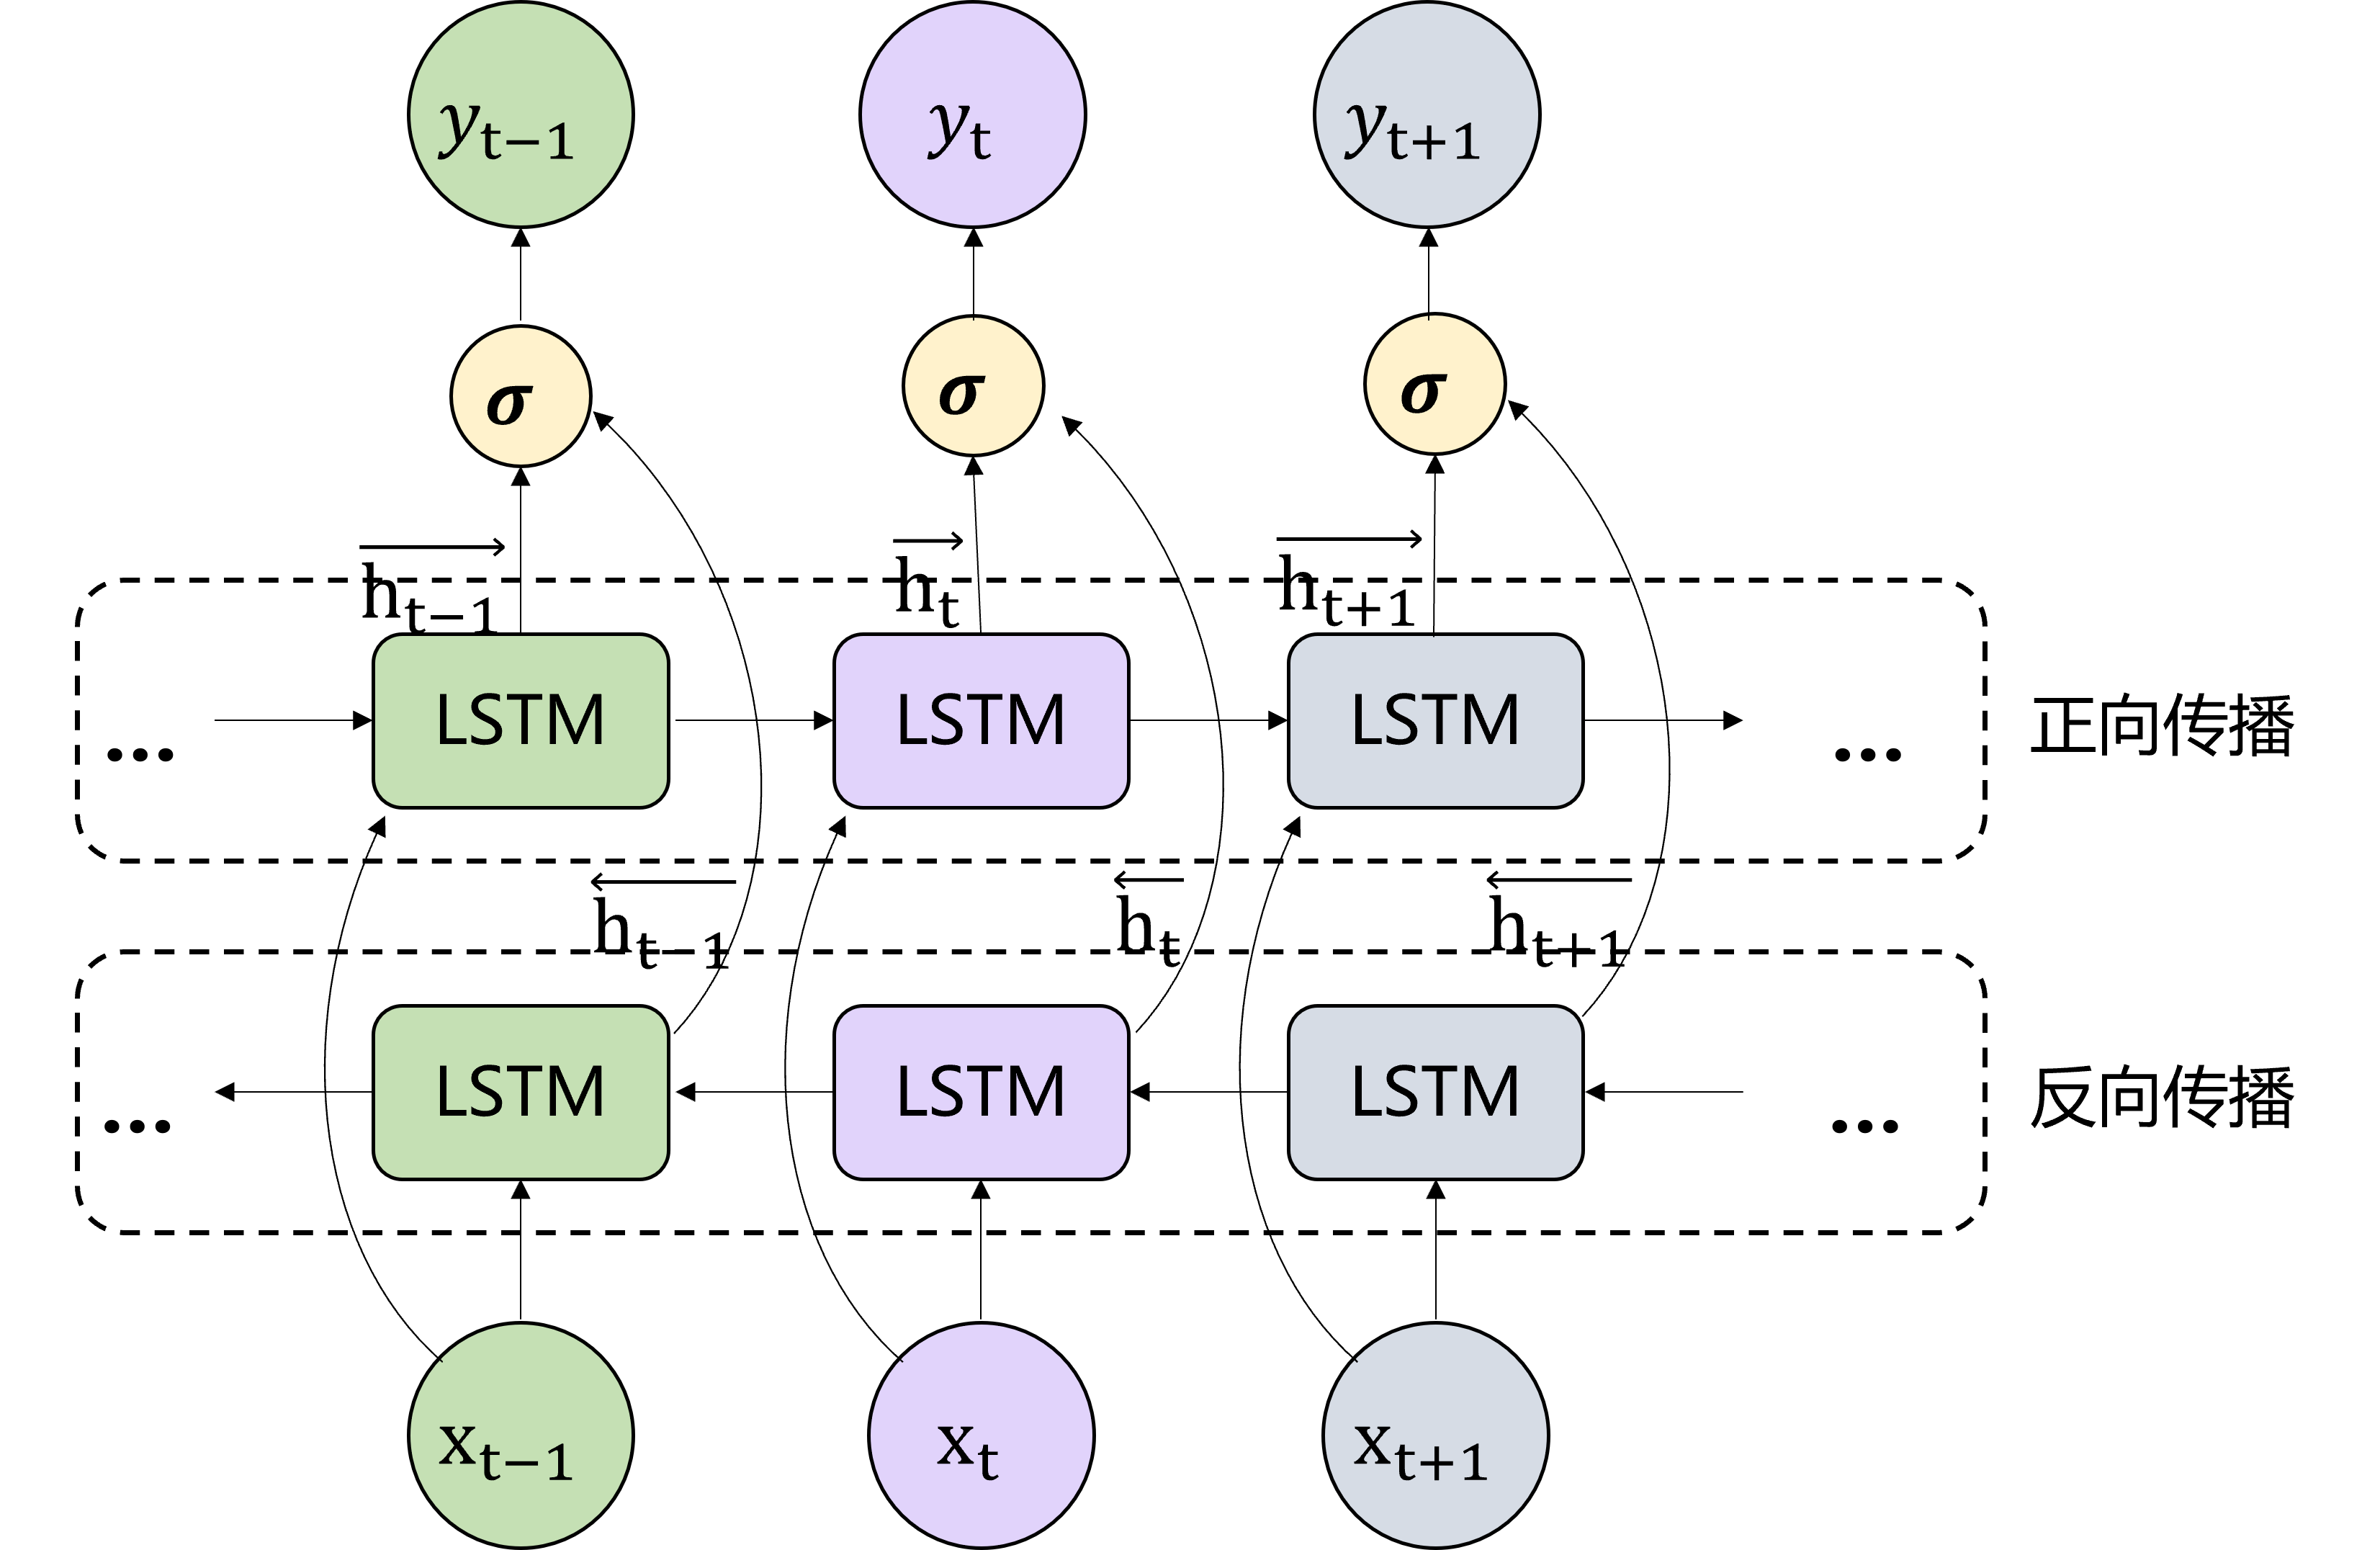
\includegraphics[width=0.65\textwidth]{figures/BiLSTM}
  \caption{BiLSTM模型结构图}\label{fig:BiLSTM}
\end{figure}

令BiLSTM的$t$时刻的前向隐藏状态为$\overrightarrow{h_t}$,向前输出为$\overrightarrow{y_t}$,向后隐藏状态为$\overrightarrow{h_t}$,向后输出为$\overleftarrow{y_t}$,输出层参数是$W_0$与$b_0$,则当前状态$\overrightarrow{y_t}$和$\overleftarrow{y_t}$可以通过公式\ref{e3.5}计算.
\begin{equation}\label{e3.5}
  \begin{split}
    \overrightarrow{y_t} &= W_0 \cdot LSTM\left(x_{t},\overrightarrow{h_{t-1}}\right) + b_0
    \\
    \overleftarrow{y_t} &= W_0 \cdot LSTM\left(x_{t},\overleftarrow{h_{t-1}}\right) + b_0
  \end{split}
\end{equation}

对当前状态$\overrightarrow{y_t}$和$\overleftarrow{y_t}$进行拼接可以得到当前$t$时刻的最终输出$y_t$,如公式\ref{e3.6}所示。
\begin{equation}\label{e3.6}
  \begin{split}
    y_t = \overrightarrow{y_t} \oplus\overleftarrow{y_t}
  \end{split}
\end{equation}

\section{Token表征方法具体实现}
\label{sec:Tokenachieve}
在介绍具体实现之前,本节首先给出Token表征方法的输入:经过\ref{subsec:Preprocess}小节的代码预处理阶段,得到示例代码片段\ref{fig:code}对应的Token序列,如图\ref{fig:tokencode}所示。
\begin{figure}[H] 
  \centering  %居中
  \subfigure[代码片段1对应的Token序列]{   %第一张子图
      \centering    %子图居中
      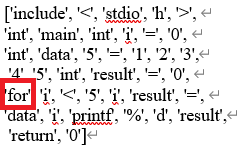
\includegraphics[width=0.3\textwidth]{figures/token1} 
      \label{fig:token1} %引用标签
  }
  \subfigure[代码片段2对应的Token序列]{ %第二张子图
      \centering    %子图居中
      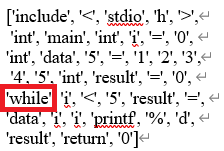
\includegraphics[width=0.3\textwidth]{figures/token2}
      \label{fig:token2} %引用标签
  }
  \subfigure[代码片段3对应的Token序列]{ %第三张子图
      \centering    %子图居中
      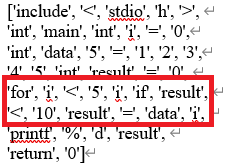
\includegraphics[width=0.3\textwidth]{figures/token3}
      \label{fig:token3} %引用标签
  }
  \caption{示例源代码对应的Token序列}    %大图名称
  \label{fig:tokencode}    %图片引用标记
\end{figure}

接下来,本章提出的基于预训练辅助模型的Token表征学习方法的实现如图\ref{fig:token}所示。该方法的输入是一对代码片段$C_{a},C_{b}$对应的Token序列,表示为$\left( w_{1}^{a},w_{2}^{a},\ldots,w_{m}^{a}\right)$ 和 $\left( w_{1}^{b},w_{2}^{b},\ldots,w_{n}^{b} \right)$,输出是$C_{a},C_{b}$对应的属性特征向量 $V_{a}^{Token},V_{b}^{Token}$,整体采用Siamese架构,两个子网络共享权值,从下到上,主要包括预训练辅助词嵌入、Token代码表征两个阶段。

\begin{figure}[H]
  \centering
  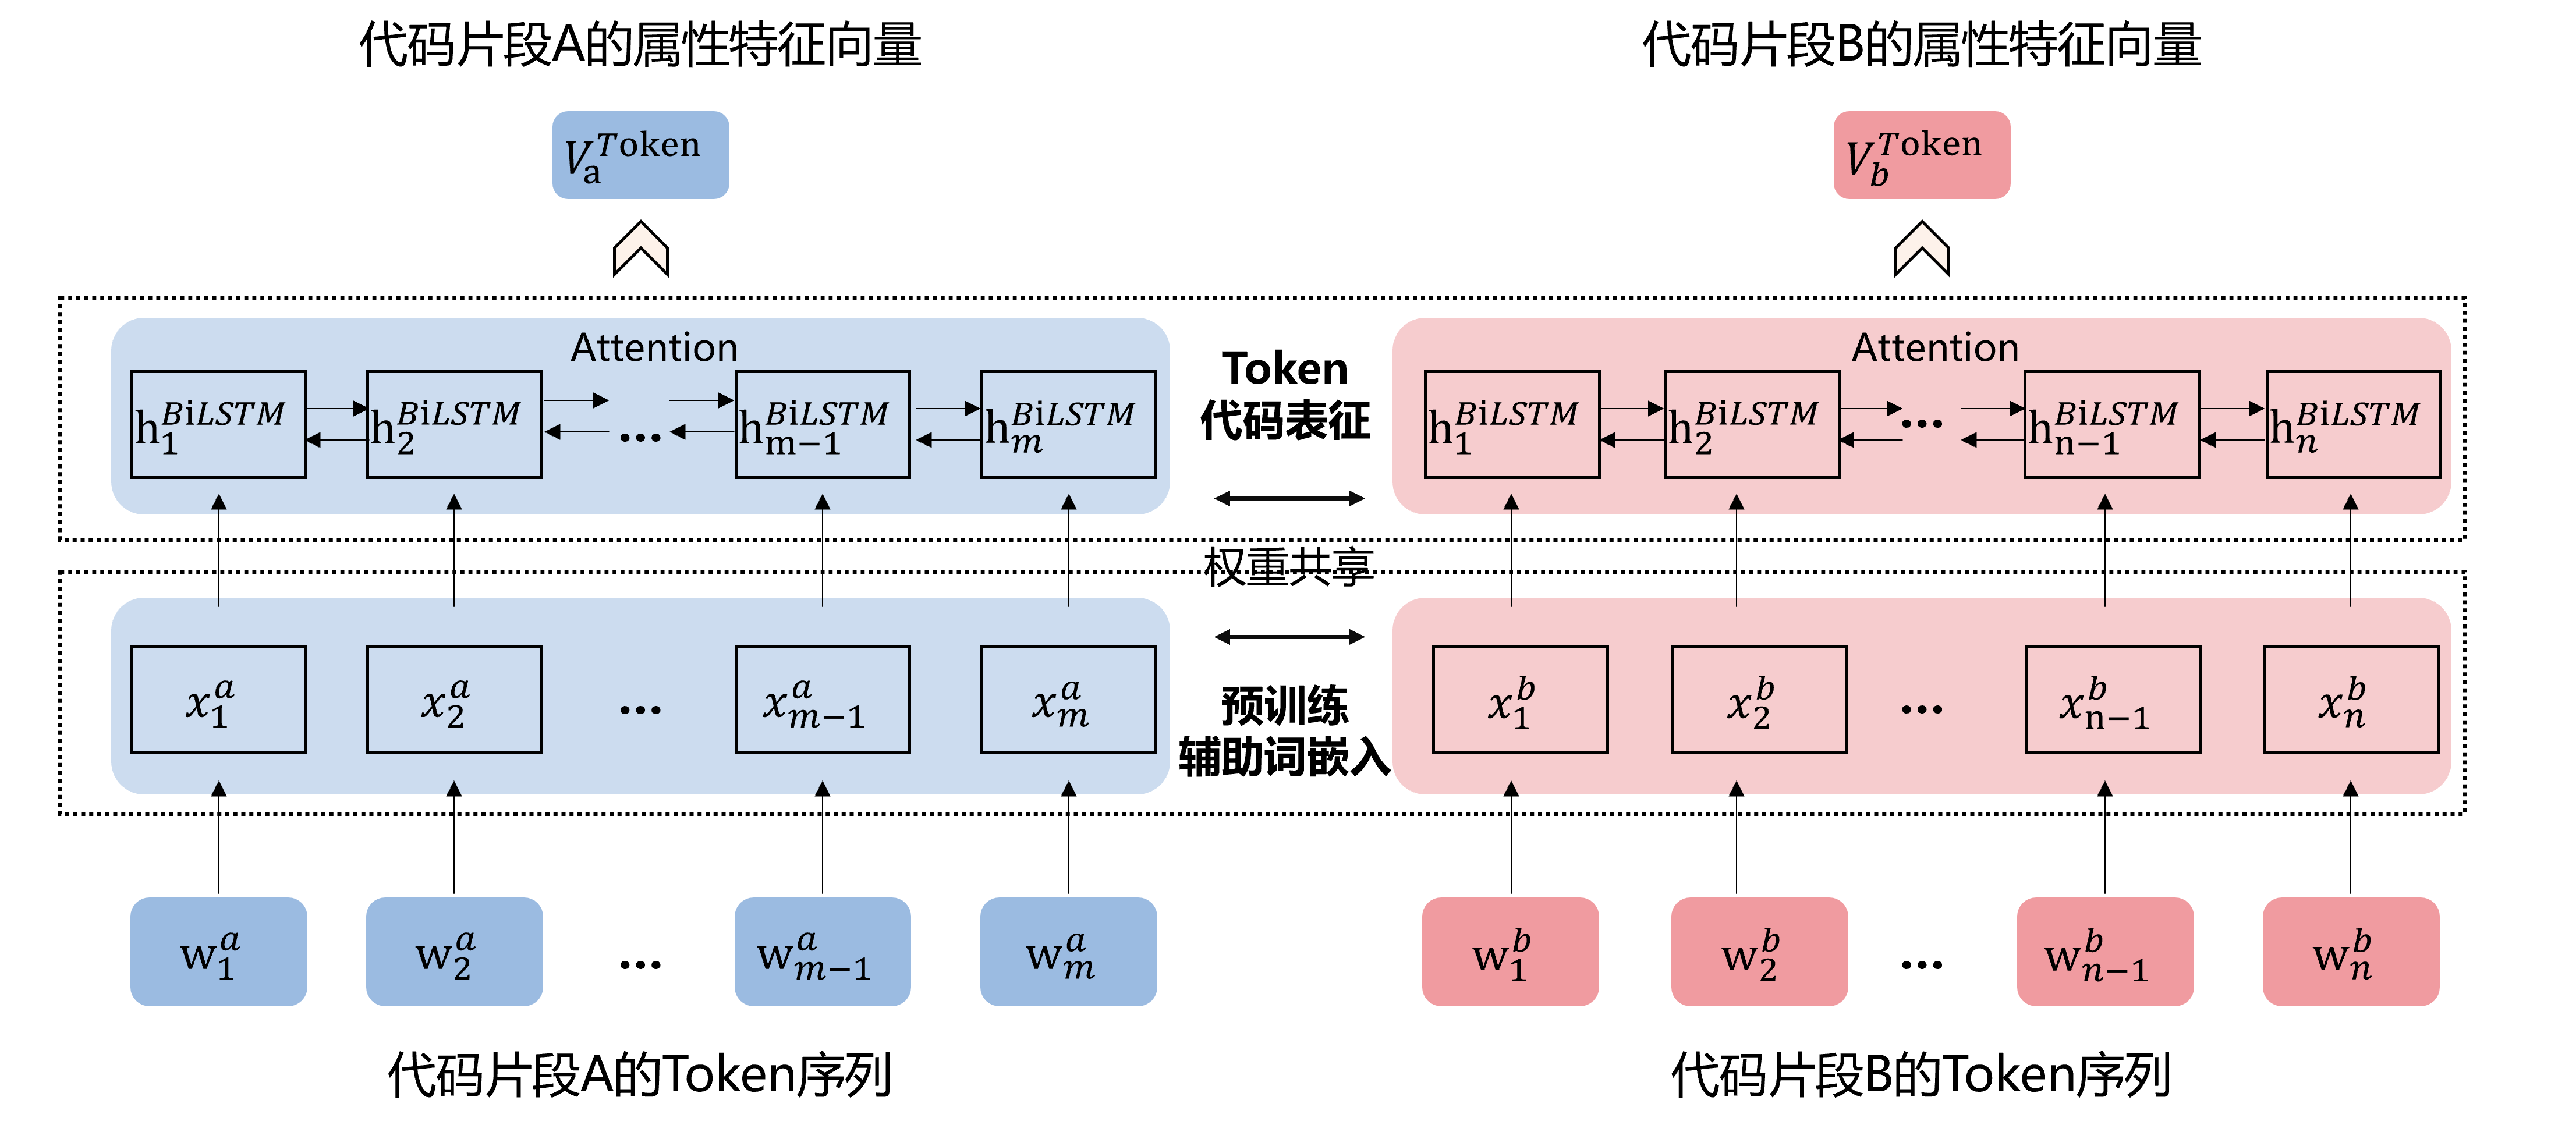
\includegraphics[width=0.9\textwidth]{figures/token}
  \caption{基于预训练辅助模型的Token表征学习方法实现}\label{fig:token}
\end{figure}

具体来说,在预训练辅助词嵌入阶段,对于代码片段$C_{a}$,经过分割得到的Token序列$\left( w_{1}^{a},w_{2}^{a},\ldots,w_{m}^{a}\right)$,($m$是代码片段A的长度),然后在词汇表$E_{w}$中查找每个Token对应的向量,将所有的token $w_{i}^{a} \left(i \in [1,m]\right)$ 转化为密集向量。其中查找词汇表$E_{w}$已经经过代码语料库使用相邻单元迭代算法ATIA基于Word2vec模型进行预训练,在模型中是固定的。其查找过程可以表示为公式\ref{e3.7}:

\begin{equation}\label{e3.7}
  \begin{split}
  x_{i}^{a} = lookup\_Token \left(w_{i}^{a} ,E_{w} \right)
  \end{split}
\end{equation}

经过嵌入阶段的预训练后,代码片段$C_{a}$生成了序列$\left( x_{1}^{a},x_{2}^{a},\ldots,x_{m}^{a}\right)$。使用同样的嵌入方式,可以得到对于Token序列$\left( w_{1}^{b},w_{2}^{b},\ldots,w_{n}^{b}\right)$,($n$是代码片段B的长度)的向量表示$\left( x_{1}^{b},x_{2}^{b},\ldots,x_{n}^{b} \right)$。

在Token代码表征阶段,将代码向量的Token序列作为输入,使用BiLSTM模型进行编码。处理过程分为两个步骤,如公式\ref{e3.8}所示:

\begin{equation}\label{e3.8}
  \begin{split}
    h_{1}^{aBiLSTM},h_{2}^{aBiLSTM},\ldots,h_{n}^{aBiLSTM} = BiLSTM \left(x_{1}^{a},x_{2}^{a},\ldots,x_{m}^{a}\right) \\
    V_{a}^{Token} = Attention \left( h_{1}^{aBiLSTM},h_{2}^{aBiLSTM},\ldots,h_{n}^{aBiLSTM} \right)
  \end{split}
\end{equation}

经过嵌入阶段的预训练后,每一个Token $w_{i}^{a}$ 都被转换为一个密集向量$x_{i}^{a}$,经过BiLSTM编码后,生成了$h_{i}^{aBiLSTM}$,然后经过Attention层的总结后,生成了$V_{a}^{Token}$作为代码片段$C_{a}$的最终Token表示,即属性特征向量。
同样,可以使用相同的计算以$\left( x_{1}^{b},x_{2}^{b},\ldots,x_{n}^{b} \right)$作为输入为代码片段$C_{b}$计算$V_{b}^{Token}$。

\section{实验验证}
\label{sec:TokenExperiment}
为了验证基于预训练辅助模型的Token表征方法的有效性,本节展开实验验证。首先,介绍了实验整体的环境配置、数据集,以及实验评估指标;接着,对基于预训练模型的Token表征方法进行了消融实验。

\subsection{实验环境}
\label{subsec:Environment}
本章的实验验证均运行于Linux系统下,其系统硬件配置如表\ref{tab:environment}所示。
\begin{table}[H]
  \centering
  \caption{实验环境配置} 
  \label{tab:environment}
  \begin{tabular*}{0.5\textwidth}{@{\extracolsep{\fill}}cc}
  \toprule
    环境			&配置		\\
  \midrule
    操作系统		&Ubuntu 20.04 \\
    处理器			&Intel Core i9-12900KF × 24 \\
    内存			  &31.1G \\
    显卡			  &NVIDIA  \\
    磁盘			  &1TB \\
  \bottomrule
  \end{tabular*}
\end{table}

\subsection{实验数据集}
\label{subsec:Dataset}
为了验证预训练辅助模型在Token层面上表征学习的有效性,本文面向代码克隆检测任务对预训练辅助模型进行分析和评估,选取的实验数据为POJ104数据集。如表\ref{tab:dataset}所示,POJ104数据集是一个基于C语言所构建的大型数据集。OJ系统是一个以编程教学为目的公开评判系统,共存在104个编程问题,针对每个编程问题,学生们通过在线提交自己的代码来尝试解决,同时OJ系统将自动判断提交源代码的正确性和有效性。对于OJ系统来说,同一个问题的不同答案可以看作一对真克隆对,不同问题的答案可以视为一对假克隆对。POJ104数据集针对每一个编程问题,均提供500个学生提交源代码,即共有52000个样本。

\begin{table}[H]
  \centering
  \caption{POJ104数据集} 
  \label{tab:dataset}
  \begin{tabular*}{0.5\textwidth}{@{\extracolsep{\fill}}cc}
  \toprule
    代码			&属性		\\
  \midrule
    Dataset			&POJ104数据集 \\
    Language    &C \\
    Program			&52000 \\
    Classes			&104 \\
    Max tokens			&8737 \\
    Avg tokens			&245 \\
  \bottomrule
  \end{tabular*}
\end{table}

得到POJ104数据集后,本文首先对数据集进行初步筛选,去掉其中包含乱码的样本,共得到51485个源代码样本。然后对源代码进行预处理,通过深入研究并比较现有标记转换规则,发现CCLearner\cite{10.1145/1287624.1287634}对转换规则进行了实验评估,验证各个标记的有效性,因此本文参考CCLearner\cite{10.1145/1287624.1287634}这篇文献的转换规则,对标识符进行了归一化处理。具体地,保留IF、For等关键词,数字常量值用NUM替代,字符串用String替代等。删除样本中包含的空白行和注释等多余代码,并将数据集保存到一个program.pkl文件中,program.pkl文件中一共包含51485行×3列的数据集,每一行数据代表一个源代码样本,第一列为源代码id,第二列保存源代码样本code,第三列为源代码的标签label,即属于哪一个编程问题。

接着,本文随机两两组合同一标签label的源代码,组成5200个真克隆对,随机组合不同标签的源代码组成44800个假克隆对,一共给包含50000个克隆对,并将其保存到oj\_clone\_ids.pkl文件中,oj\_clone\_ids.pkl文件中一共包含50000行×3列的数据集,每一行数据代表一个克隆对样本,第一列为源代码id1,第二列为源代码id2,第三列为克隆对的标签label,真克隆对标签为1,假克隆对标签为0。最后,依据随机种子将数据集按照3:1:1划分为训练集、测试集、验证集,其中的正负样本数如下表\ref{tab:ClonePairs}所示。

\begin{table}
  \centering
  \caption{本文预处理后的POJ104数据集正负样本数} 
  \label{tab:ClonePairs}
  \begin{tabular*}{0.8\textwidth}{@{\extracolsep{\fill}}cccc}
  \toprule
    数据集			&真克隆对		&假克隆对		&克隆对数 \\
  \midrule
    训练集train			&3162	  &26838		&30000 \\
    测试集test			&1022		&8978		  &10000 \\
    验证集dev			  &1016		&8984		  &10000 \\
    总计            &5200	  &44800	  &50000 \\
  \bottomrule
  \end{tabular*}
\end{table}

\subsection{评估指标}
\label{subsec:Index}
代码克隆检测问题是二分类问题,因此本文采用精确率(Precision)、召回率(Recall)、F1值三个评估指标来度量实验结果,其中使用了混淆矩阵中的TP、FN、FP、TN,如表\ref{tab:ConfusionMatrix}所示。

\begin{table}[H]
  \centering
  \caption{分类问题的混淆矩阵} 
  \label{tab:ConfusionMatrix}
  \begin{tabular*}{0.7\textwidth}{@{\extracolsep{\fill}}ccc}
  \toprule
  \multirow{2}{*}{实际值} & \multicolumn{2}{c}{预测值} \\
  \cmidrule{2-3} 
  \multirow{2}{*}{} & 正样本(P) & 负样本(N) \\
  \midrule
    正样本(P)			&TP	  &FN		 \\
    负样本(N)			&FP		&TN		 \\
  \bottomrule
  \end{tabular*}
\end{table}

其中,混淆矩阵中的真阳性、假阳性、真阴性、假阴性代表的含义如下:

真阳性(True Positive, TP):样本实际为正样本,并且被模型预测为正样本,即实际上标记为真克隆对并且被检测出来为真克隆对的代码对。
 
假阳性(False Positive, FP):样本实际为负样本,但是被模型预测为正样本,即实际上标记为假克隆对但是被检测出来为真克隆对的代码对。
 
假阴性(False Negative, FN):样本实际为正样本,但是被模型预测为负样本,即实际上标记为真克隆对但是被检测出来为假克隆对的代码对。
 
真阴性(True Negative, TN):样本实际为负样本,并且被模型预测为负样本,即实际上标记为假克隆对并且被检测出来为假克隆对的代码对。

精确率(Precision)表示正确检测到的代码克隆数量占全部预测为代码克隆的比例,计算公式如\ref{e6}所示:
\begin{equation}\label{e6}
  Precision = \frac{TP}{TP+FP} 
\end{equation}

召回率(Recall)表示正确检测到的代码克隆数量占总体实际代码克隆数量的比例,计算公式如\ref{e7}所示:
\begin{equation}\label{e7}
  Recall = \frac{TP}{TP+FN} 
\end{equation}

精确率(Precision)和召回率(Recall)指标有时候会出现的矛盾的情况,这样就需要综合考虑两者的表现,最常见的方法就是F1,精确率和召回率的加权调和平均,用于评价分类模型的好坏。计算公式如\ref{e8}。
\begin{equation}\label{e8}
  F1 = \frac{2*Precision*Recall}{Precision+Recall} 
\end{equation}

\subsection{实验结果}
\label{subsec:TokenResult}
(1) 预训练语料库规模的实验结果

为了探究预训练语料库规模对Token表征实验结果的影响,本文选取POJ104数据集中部分数据进行预训练,基于相邻单元迭代算法构造预训练语料库。具体地,在\ref{subsec:Dataset}数据库中随机选取了100对、200对、500对代码克隆对作为预训练数据集,构造预训练语料库,对Token表征模型进行预训练。具体实验结果如表\ref{tab:category}所示。

\begin{table}[H]  
  \centering  
  \caption{预训练语料库规模对实验结果的影响}   
  \label{tab:category}  
  \begin{tabular*}{0.9\textwidth}{@{\extracolsep{\fill}}ccccc}  
  \toprule
  \multirow{2}{*}{预训练数据集规模} & \multirow{2}{*}{词表长度} & \multicolumn{3}{c}{OJClone} \\
  \cmidrule{3-5} 
   & & 准确率(\%) & 召回率(\%) & F1值(\%)  \\  
  \midrule 
  100对	&231		& xxx	& xxx	& xxx		 \\  
  300对	&444		& xxx	& xxx	& xxx		\\  
  500对	&600 	& 89.74	& 87.84	& 88.78	\\  
  \bottomrule  
  \end{tabular*}  
\end{table}
从表\ref{tab:category}可以看出, 随着预训练语料库的增大, 代码克隆检测任务的F1值呈现上升趋势, 即对代码克隆的检测效果会不断增强。考虑到需要预留出足够的答案样本用来构造训练集和测试集, 最终选择500对作为C语言实验中的预训练数据集大小。

(2) Token表征模型实验结果

为了探究Token表征模型AttBiLSTM对实验结果的影响,本文基于预训练辅助的基础上,将AttBiLSTM模型与LSTM与BiLSTM模型进行对比,结果如表\ref{tab:category2}所示。其中LSTM、BiLSTM模型基于Pytorch1.10实现,其参数设置为:

词嵌入层:将大小为600的词汇表映射到128维的向量空间。
双向LSTM层:双向的LSTM单元堆叠而成,输入特征的维度与嵌入层匹配为104层,隐藏层维度设置104,由于设置为双向,因此输出维度为104*2=208层。
全连接层:208层的输入映射到1维的输出中
sigmoid层:激活函数,将全连接层的输出转换到0到1之间的概率值。

模型的优化器为Adam优化器,学习率设置为0.0001,dropout 为0.1,epochs为50,参数的确定是通过多次调试后选择最优参数作为最后的结果。

\begin{table}[H]  
  \centering  
  \caption{Token表征模型对实验结果的影响(\%)}   
  \label{tab:category2}  
  \begin{tabular*}{0.9\textwidth}{@{\extracolsep{\fill}}cccc}  
  \toprule  
  表征模型 & 准确率(\%) & 召回率(\%) & F1值(\%)  \\  
  \midrule  
  LSTM			& xxx	& xxx	& xxx		 \\  
  BiLSTM			& xxx	& xxx	& xxx		 \\  
  AttBiLSTM			& 89.74	& 87.84	& 88.78		\\  
  \bottomrule  
  \end{tabular*}  
\end{table}
从表\ref{tab:category}可以看出, 随着预训练语料库的增大, 克隆检测任务的F1值呈现上升趋势, 即对代码克隆的检测效果会不断增强. 考虑到需要预留出足够的答案样本用来构造训练集和测试集, 最终选择AttBiLSTM模型作为Token表征模型。

\section{本章小结}
\label{sec:Summary3}
本章主要对RLCCD中基于预训练辅助模型的Token表征学习方法的设计与实现进行详细阐述。首先介绍了Token维度的研究动机,其次介绍了Token表征学习的方法设计,具体论述了其整体框架、预训练辅助模型、表征学习,接着开展实验验证,结果表明了此方法的有效性和模型的准确性。
